\documentclass[sigconf]{acmart}
%% \documentclass[manuscript,screen]{acmart}

%% \BibTeX command to typeset BibTeX logo in the docs
\AtBeginDocument{%
  \providecommand\BibTeX{{%
    \normalfont B\kern-0.5em{\scshape i\kern-0.25em b}\kern-0.8em\TeX}}}

%%\acmSubmissionID{123-A56-BU3}

%%\citestyle{acmauthoryear}

%%
%% end of the preamble, start of the body of the document source.
\begin{document}

\title{Milestone 1 -- Unsupervised Learning}

\author{Maciej Nalepa}
\affiliation{}
\email{maciej.nalepa@alu.uclm.es}

\author{Piotr Maliszewski}
\affiliation{}
\email{piotr.maliszewski@alu.uclm.es}

\author{Gökay Iseri}
\affiliation{}
\email{gokay.iseri@alu.uclm.es}

\author{Başar Milli}
\affiliation{}
\email{basar.milli@alu.uclm.es}

\renewcommand{\shortauthors}{Nalepa Maliszewski Iseri Milli}

\begin{abstract}
The purpose of this work is to explore the environmental data collected by various U.S.
Federal Government Agencies from two cities ( San Juan, Puerto Rico and Iquitos, Peru) to
gain a better understanding of the Denge Spread Phenomena.
These data are from a competition of the site DrivenData. Training data will be used.
The overall objective is to use unsupervised learning techniques to make a preliminary exploration of the data and to extract conclusions from discarded elements, etc. The specific
objectives are as follows:

\begin{enumerate}
    \item Identification of outliers elements (weeks) in the dataset.
    \item Use clustering algorithms to identify groups and characterize them.
    \item (optional) Feature Selection using clustering algorithms.
\end{enumerate}

\end{abstract}

%%
%% http://dl.acm.org/ccs.cfm
%%
\begin{CCSXML}
<ccs2012>
   <concept>
       <concept_id>10010147.10010257</concept_id>
       <concept_desc>Computing methodologies~Machine learning</concept_desc>
       <concept_significance>500</concept_significance>
       </concept>
 </ccs2012>
\end{CCSXML}

\ccsdesc[500]{Computing methodologies~Machine learning}

\keywords{machine learning, unsupervised}

\maketitle

%
%   +++++++OUR CODE
%

\section{Introduction}
In this project we explore Unsupervised Learning methods.
We were working on DrivenData DengAI: Predicting Disease Spread competition dataset.
Exactly our group was focused on finding relations among the data from San Juan between years 1992 - 1998.

The code and source files are available at  \url{https://github.com/GummyBearStudioTeam/ESI_MLTechniques}.

\subsection{Correlation factor}
The data is not strongly correlated except the temperature fields.

\begin{figure}[h]
    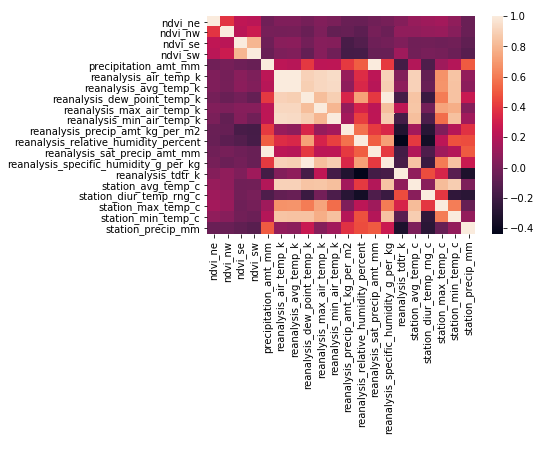
\includegraphics[width=\linewidth]{correlation.png}
    \centering
    \caption{Unprocessed data correlation matrix}
    %\Description{}
\end{figure}

\section{Dimensionality Reduction}
\begin{figure}[h]
    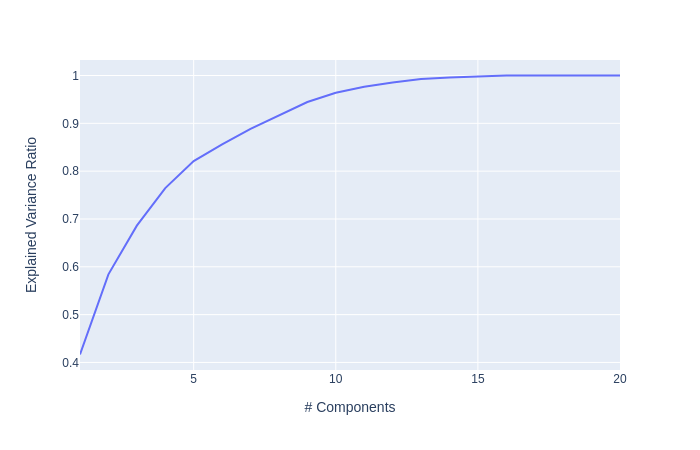
\includegraphics[width=\linewidth]{pca.png}
    \centering
    \caption{PCA: Explained variance ratio}
    %\Description{}
\end{figure}

According to the explained variance ratio by projecting the data to 10 dimensions, we can preserve arround 96\% of information. That allows us to keep a lot of information by reducing total number of dimensions by half.

\section{Outlier Identification}

\begin{table}
  \caption{DBSCAN results with specific epsilon.}
  \label{tab:eps}
  \begin{tabular}{rll}
    \toprule
    $epsilon$ & clusters & outliers \\
    \midrule
    1.2  & 0  & 364 \\
    1.4  & 1  & 360 \\
    1.6  & 4  & 346 \\
    1.8  & 8  & 297 \\
    2.0  & 5  & 252 \\
    2.2  & 5  & 180 \\
    2.4  & 3  & 134 \\
    2.6  & 2  & 91  \\
    2.8  & 2  & 58  \\
    3.0  & 1  & 37  \\
    3.2  & 1  & 29  \\
    3.4  & 1  & 17  \\
    3.6  & 1  & 10  \\
    3.8  & 1  & 6   \\
    4.0  & 1  & 5   \\
    4.2  & 1  & 3   \\
    4.4  & 1  & 3   \\
    4.6  & 1  & 2   \\
    4.8  & 1  & 2   \\
    \bottomrule
\end{tabular}
\end{table}

\begin{figure}[h]
    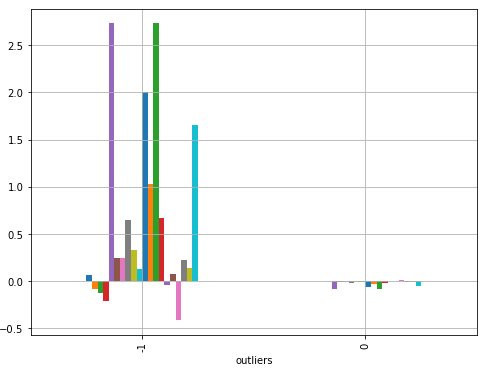
\includegraphics[width=\linewidth]{outliers-mean.png}
    \centering
    \caption{Outliers' mean}
    %\Description{}
\end{figure}

Features that have the biggest impact on outliers are all of the measures of precipitation(Highest purple, green and blue bars). Differences are noticeable so we decided not to take them into consideration in further analysis.

\section{Clustering}
    The number of cluster ($k$) has been chosen as 3, because higher values reduce Silhouette score significantly.
    \begin{figure}[h]
    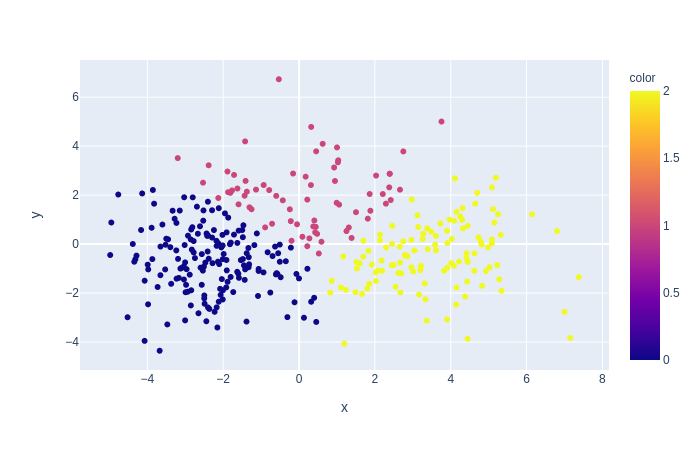
\includegraphics[width=\linewidth]{kmeans.png}
    \centering
    \caption{K-means clusters projected into 2D}
    %\Description{}
\end{figure}
\subsection{K-means}
    \begin{figure}[h]
        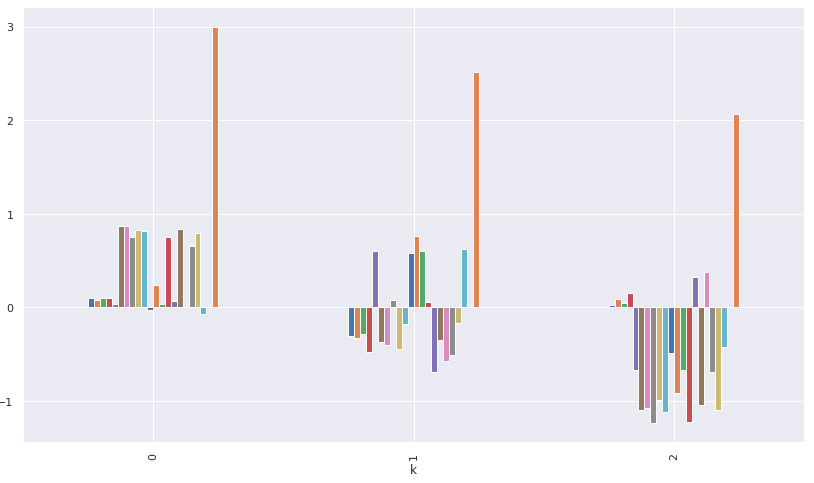
\includegraphics[width=\linewidth]{kmeans-mean.png}
        \centering
        \caption{K-means - mean diagram}
        %\Description{}
    \end{figure}
    \begin{enumerate}
        \item Group 0 has greater mean of precipitation while having lower temperatures. Humidity is around the average. This group could be labelled as having low temperature with big precipitations
        \item Group 1 has an average precipitation, but it's climate is more humid and temperatures are higher than a mean of the whole data. This group could be labelled as as having high temperature with big precipitations
        \item Group 2 has noticeable the biggest humidity from the previous groups. Both temperature and precipitation are low. Almost all features deviate from the mean significantly. This group could be labelled as having low temperature with small precipitations.
    \end{enumerate}
    
\subsection{Hierarchical}

    \begin{figure}[h]
        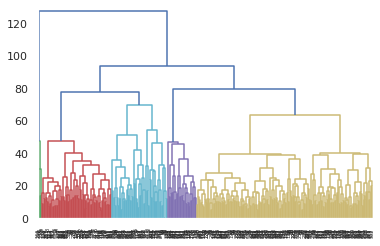
\includegraphics[width=\linewidth]{dendogram-70.png}
        \centering
        \caption{Dendogram}
        %\Description{}
    \end{figure}
    
     The clusters have been created by cutting a tree at the height 70. It was a value that allowed us to make some bigger insight about the data. Different value either could group everything in gigantic groups or would be too fragmented.
     
    \begin{figure}[h]
        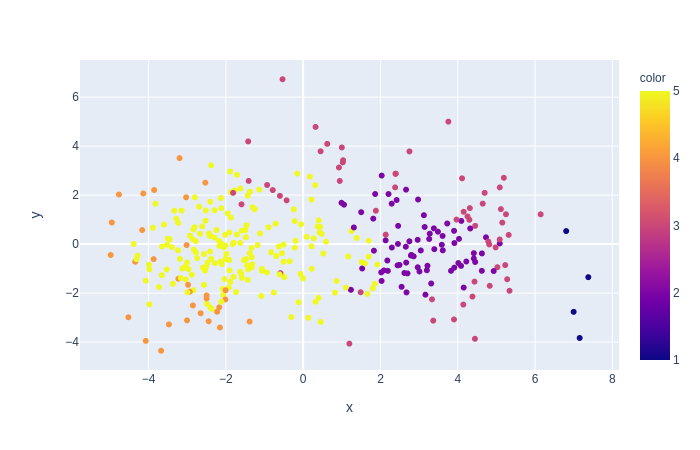
\includegraphics[width=\linewidth]{hierarchical.png}
        \centering
        \caption{Hierarchical clustering PCA chart}
        %\Description{}
    \end{figure}
    
\begin{enumerate}
        \item Group 0 is characterised by  a greater diurnal temperature range. Winds are above the average when temperatures precipitation and humidity are very low but the whole group is small, so it's mean should not be used to extract further details from it.
        \item Groups 1 and 2 are quite similar. The biggest difference is that the 1st group has lower precipitation when the 2nd one has a precipitation around the global average. Both have low temperatures and humidity.
        \item Group 3 - In that group all of the features are above the average. It seems that the temperature is the most significant factor. It is the only representative group (without taking into consideration the 0th group) where strong winds occurs.
        \item Group 4 - In that group most of features are above the average, but a deviation is smaller than in the 3rd group. What characterise that group as well are winds which force is about the average
\end{enumerate}


\section{Feature selection}
Basing on hierarchical clustered data we propose following features:
\begin{itemize}
    \item \texttt{ndvi\_ne}
    \item \texttt{ndvi\_nw}
    \item \texttt{ndvi\_se}
    \item \texttt{ndvi\_sw}
    \item \texttt{precipitation\_amt\_mm}
    \item \texttt{reanalysis\_precip\_amt\_kg\_per\_m2}
    \item \texttt{reanalysis\_specific\_humidity\_g\_per\_kg}
\end{itemize}
Mean values of these features in each cluster deviate from each other significantly.

\section{Refinement}
Columns allowing to identify the week were dropped but if they were preserved it could allow to get some conclusions manually.

Variable names for storing data could be improved, because currently they can be difficult to distinguish. (e.g. \texttt{df} and \texttt{df2})

Feature selection was performed manually by comparing charts of mean values between clusters, which should instead be performed using some numerical metrics. There was also no verification if the selected features are sufficient to distinguish the clusters in the same way.

K-means, hierarchical clustering and DBSCAN parameters can be adjusted to create different groups.

\section{Summary}
We have explored the dataset and learned how to use the unsupervised learning tools.

Scatter plots representing the clusters work the better the less clusters we create.
The resulting groups are similar when using either method of clustering, we decided to create more clusters using hierarchical method.

%
%   -------OUR CODE
%

%% The acknowledgments section is defined using the "acks" environment
%% (and NOT an unnumbered section). This ensures the proper
%% identification of the section in the article metadata, and the
%% consistent spelling of the heading.
\begin{acks}
This work is part of UCLM project of the Machine Learning Techniques subject. Group PMG.
\end{acks}

%%
%% The next two lines define the bibliography style to be used, and
%% the bibliography file.
%\bibliographystyle{ACM-Reference-Format}
%\bibliography{sample-base}

\end{document}
\endinput
%%
%% End of file `sample-xelatex.tex'.
